% \documentclass[handout]{beamer}
\documentclass[presentation]{beamer}
\usepackage{ctex}
\usecolortheme{duxing}
\usefonttheme{duxing}
\useinnertheme{duxing}
 
\usepackage[utf8]{inputenc}
\usepackage[UKenglish]{babel}
\usepackage{booktabs}
\usepackage{caption}
\usepackage{subcaption}
\usepackage{graphicx}
\usepackage{amsmath}
\usepackage{amsfonts}
\usepackage{amssymb}

\institute{
\includegraphics[height=0.7cm]{sysu_logo.png}
\includegraphics[height=0.7cm]{duxing_logo.png}}

\title{科研方法论}

\subtitle{深度学习研讨班 101 (暨绪论)}

\author{黄涛}

\date{}


\begin{document}
 
\frame{\titlepage}

\section{关于本课程}

\begin{frame}
    在谈到如果要给后进的学弟学妹一个学习的方法的话,刘路回答到:
    
    “我只有一个想法,就是看淡分数,重在兴趣。”
\end{frame}


\section{论文搜集、获取与管理}

\begin{frame}{学术搜索}
    学术搜索平台主要用于对论文的查找,对于开放获取权限的论文一般会给出论文pdf的链接。
    学术搜索引擎会显示该搜索引擎所统计到的引用这篇论文的文章数量和具体文章,也可以很方便地引用这篇文章。
\end{frame}

\begin{frame}{学术搜索}
    \begin{figure}
        \centering
        \begin{subfigure}{.5\textwidth}
              \centering
              
\includegraphics[width=0.8\linewidth]{_0.png}
              \caption{google学术}
        \end{subfigure}%
        \begin{subfigure}{.5\textwidth}
              \centering
              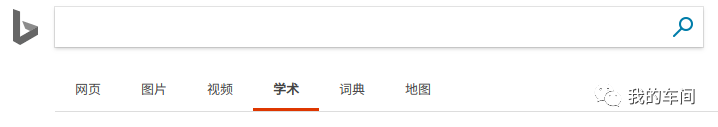
\includegraphics[width=0.8\linewidth]{_1.png}
              \caption{bing学术}
        \end{subfigure}
        \begin{subfigure}{.5\textwidth}
              \centering
              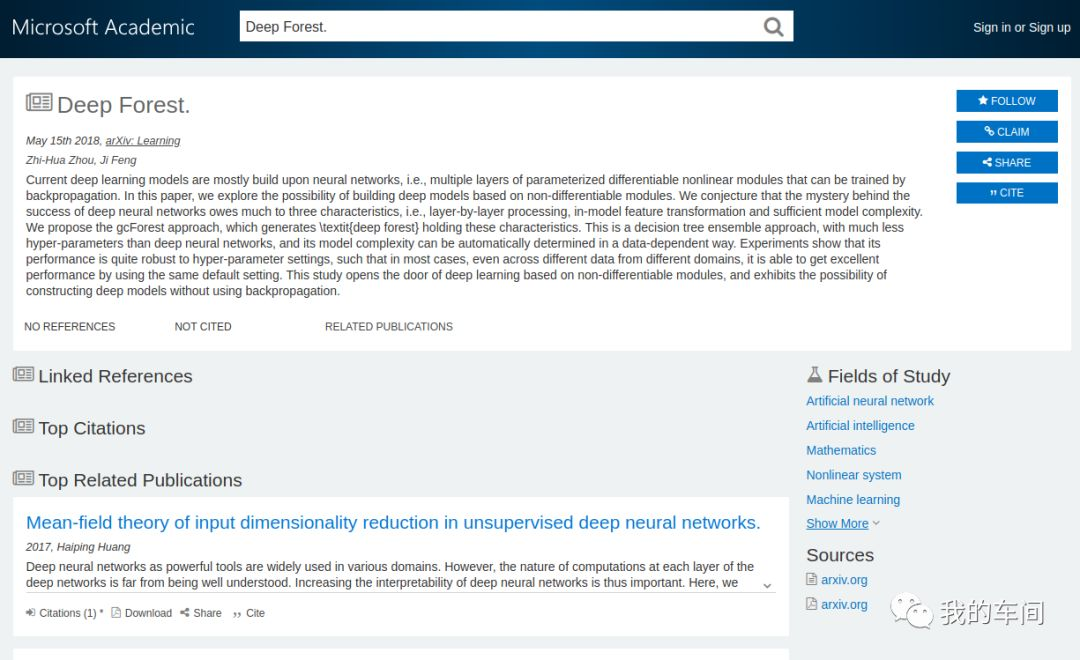
\includegraphics[width=0.8\linewidth]{_3.png}
              \caption{微软学术}
        \end{subfigure}%
        \begin{subfigure}{.5\textwidth}
              \centering
              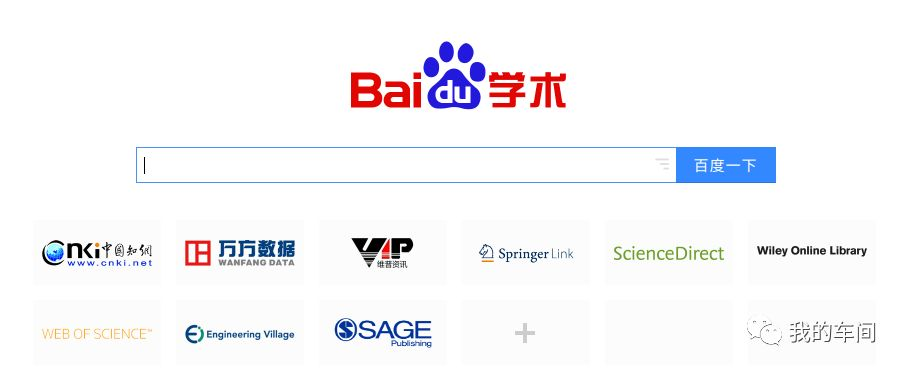
\includegraphics[width=0.8\linewidth]{_4.png}
              \caption{百度学术}
        \end{subfigure}
    \end{figure}
\end{frame}

\begin{frame}{学术搜索}
    \begin{figure}
        \centering
          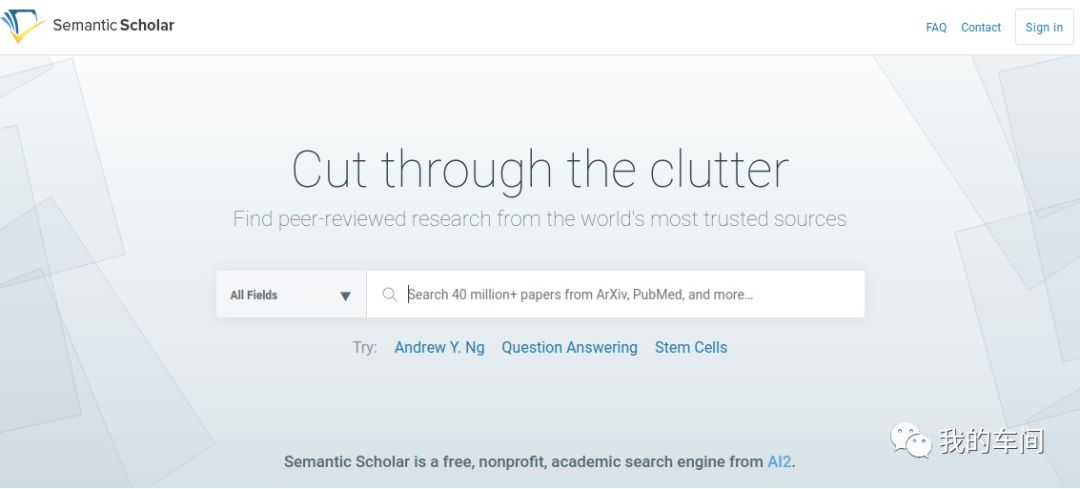
\includegraphics[width=0.8\linewidth]{_6.png}
          \caption{Semantic Scholar}
    \end{figure}
\end{frame}

\begin{frame}{学术出版}
    \begin{figure}
        \centering
          
\includegraphics[width=0.5\linewidth]{_7.png}
          \caption{arxiv}
    \end{figure}
	\textbf{arxiv}论文预发表平台是开放的获取\textbf{数学、物理和计算机}等学科论文的平台,许多的研究人员都把他们的论文都公开在这一平台上。你能够在这里找到许多公开的研究成果,特别是近几年的成果。
\end{frame}

\begin{frame}{学术出版}
    \begin{figure}
        \centering
          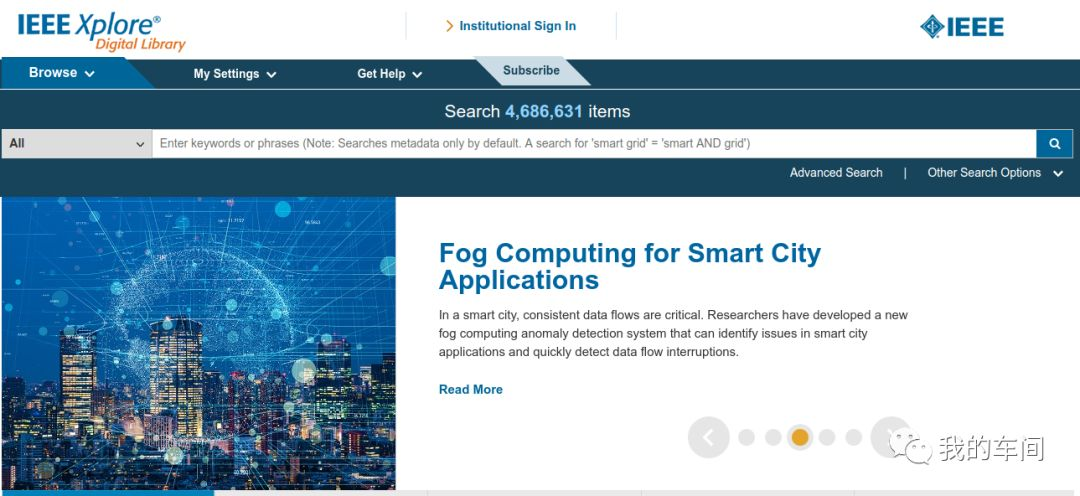
\includegraphics[width=0.7\linewidth]{_8.png}
          \caption{arxiv}
    \end{figure}
	IEEE是许多计算机/电子方向论文的版权所有者,在这里你可以找到许多计算机/电子方面的论文。
\end{frame}

\begin{frame}{学术出版}
    \begin{figure}
        \centering
          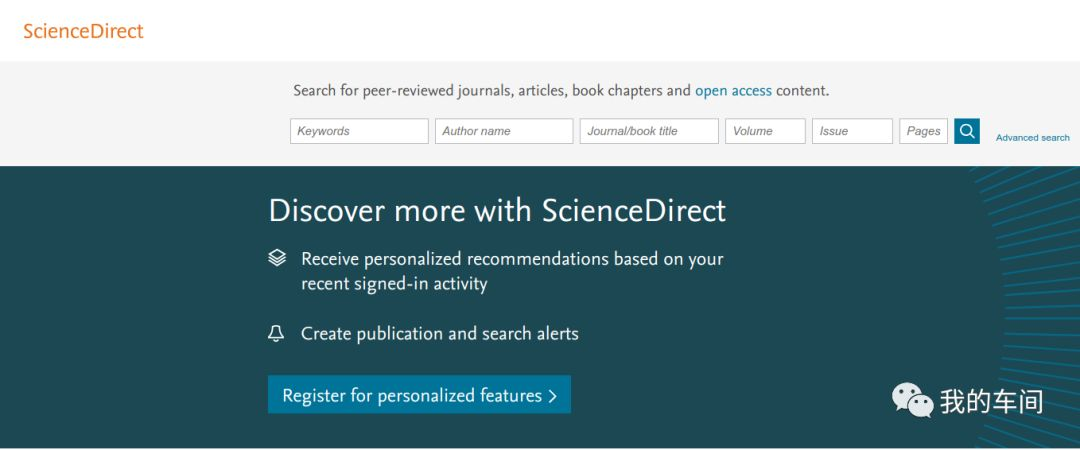
\includegraphics[width=0.7\linewidth]{_9.png}
          \caption{ScienceDirect}
    \end{figure}
	\textbf{ScienceDirect}是学术出版巨头爱思唯尔旗下的论文检索平台,在这里你可以更好的检索到由爱思唯尔出版的论文。爱思唯尔是世界上科学、技术和医学论文的主要出版者之一。
\end{frame}

\begin{frame}{学术出版}
    \begin{figure}
        \centering
          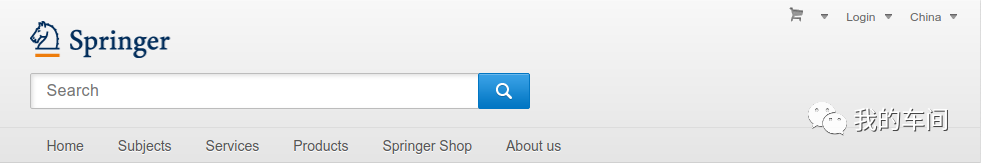
\includegraphics[width=0.7\linewidth]{_10.png}
          \caption{Springer}
    \end{figure}
	同样,\textbf{Springer}也是一大学术出版巨头,在这里你可以更方便地获取由他们出版的论文。
\end{frame}

\begin{frame}{文献获取}
	如果您没有获取论文的渠道,那么获取这些论文将会是一件不太容易的事,这里提供两个平台,能够免费获取到一些中文/英文论文:
    \begin{figure}
        \centering
        \begin{subfigure}{.5\textwidth}
              \centering
              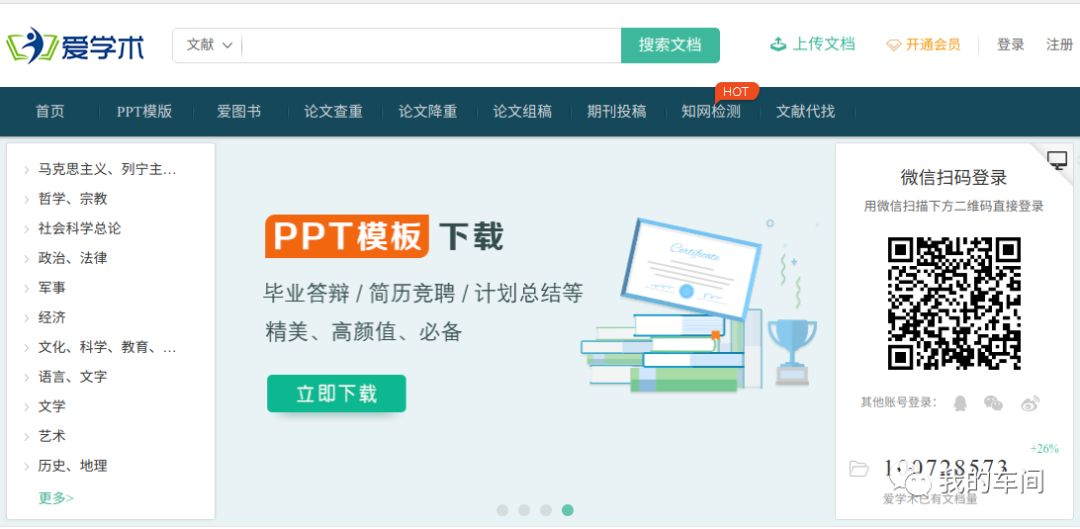
\includegraphics[width=0.8\linewidth]{_11.png}
              \caption{爱学术,您能够在此获取中文文献}
        \end{subfigure}%
        \begin{subfigure}{.5\textwidth}
              \centering
              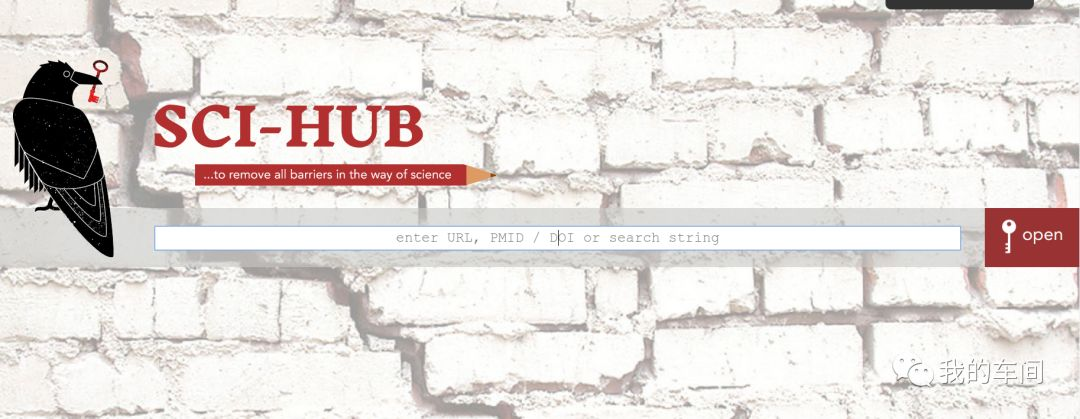
\includegraphics[width=0.8\linewidth]{_12.png}
              \caption{Sci-Hub,您能在此获取英文文献}
        \end{subfigure}
    \end{figure}
\end{frame}

\begin{frame}{文献管理}
	我相信,再也没有什么比Mendeley管理学术文献更为方便的了,作为学术出版巨头Elsevier旗下的学术管理软件,我来列举一下它的几个特点:
	\begin{itemize}
	    \item 跨平台:
        Mendeley提供网页版、桌面版(windows、mac osx以及linux)和移动版(iphone、ipad和android),而且你账户内的所有论文都是云同步的,在这个设备上添加论文后,可以很方便地在另一设备上阅读、标注以及做笔记(标注和笔记也是云同步的)。
	\end{itemize}
\end{frame}

\begin{frame}{文献管理}
    \begin{itemize}
        \item 导入pdf即可生成论文信息:
        \begin{figure}
            \centering
              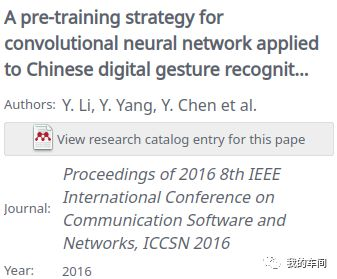
\includegraphics[width=0.5\linewidth]{_14.png}
              \caption{软件自动生成的信息}
        \end{figure}
    \end{itemize}
\end{frame}
\begin{frame}{文献管理}
    \begin{itemize}
        \item 智能推送相关文献
        \begin{figure}
            \centering
              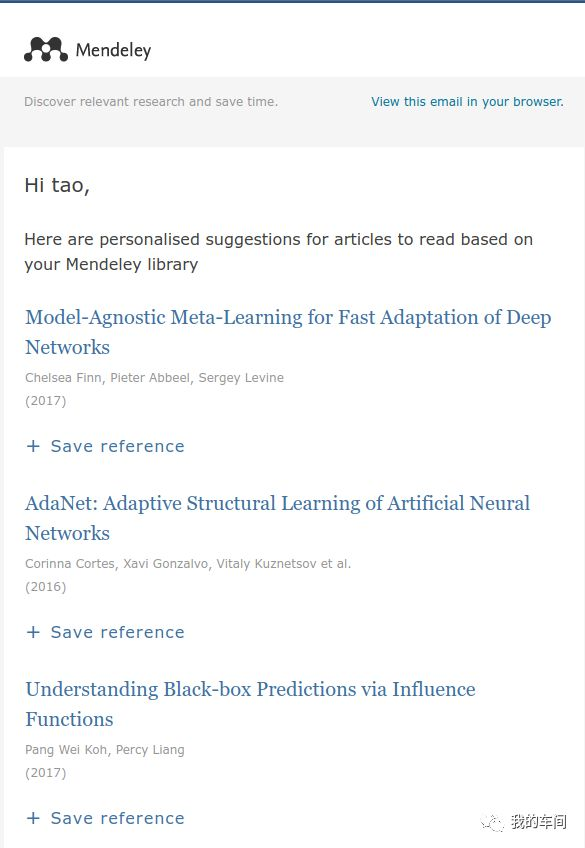
\includegraphics[width=0.3\linewidth]{_15.png}
              \caption{智能推送的文献}
        \end{figure}
    \end{itemize}
\end{frame}

\section{深度学习}
\begin{frame}{神经网络}
    \begin{figure}
        \centering
          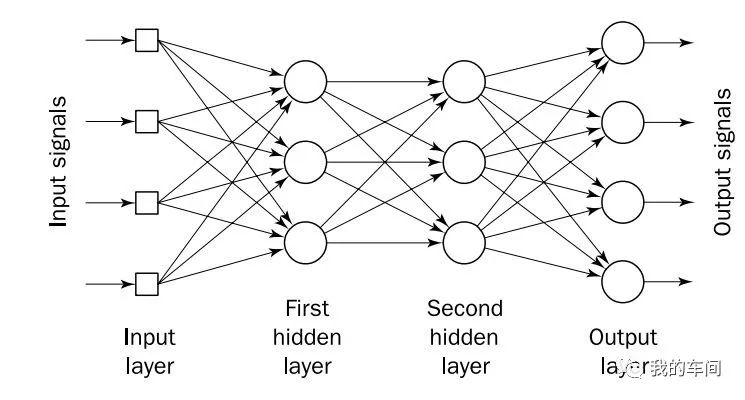
\includegraphics[width=0.8\linewidth]{2_0.jpg}
          \caption{神经网络}
    \end{figure}
    通常来说,神经网络由输入层(Input Layer)、输出层(Output Layer)和它们之间的隐含层(Hidden Layer)所构成。
\end{frame}

\begin{frame}{卷积神经网络}
    \begin{figure}
        \centering
          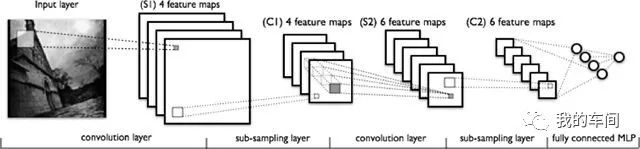
\includegraphics[width=0.8\linewidth]{2_1.jpg}
          \caption{卷积神经网络}
    \end{figure}
    卷积神经网络一般由三个类型的层构成:卷积层(Convolution Layer)、池化层(Pooling Layer)(又被称为下采样层(Sub-sampling Layer))和全连接层(Fully-connected Layer)。
\end{frame}

\begin{frame}{卷积}
    \begin{figure}
        \centering
          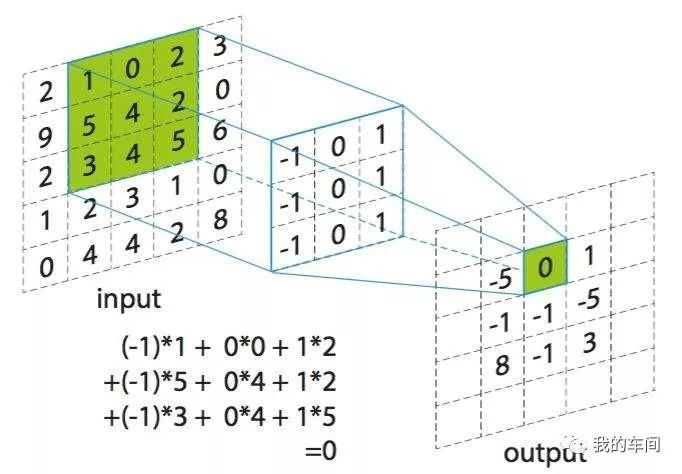
\includegraphics[width=0.7\linewidth]{2_2.jpg}
          \caption{卷积}
    \end{figure}
    离散的二维卷积操作通常可以表示为该像素及其周围像素乘以它们各自相对位置对应权值(Weights)的和。权值矩阵被称为卷积核(Kernels)。
\end{frame}

\begin{frame}{循环神经网络}
    \begin{figure}
        \centering
          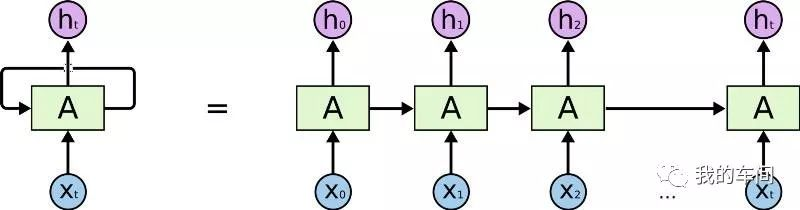
\includegraphics[width=0.8\linewidth]{2_3.jpg}
          \caption{循环神经网络}
    \end{figure}
    循环神经网络每一个时刻的状态都由其前一时刻的状态和当前时刻的输入所计算出。
\end{frame}

\begin{frame}{GPU}
    \begin{figure}
        \centering
          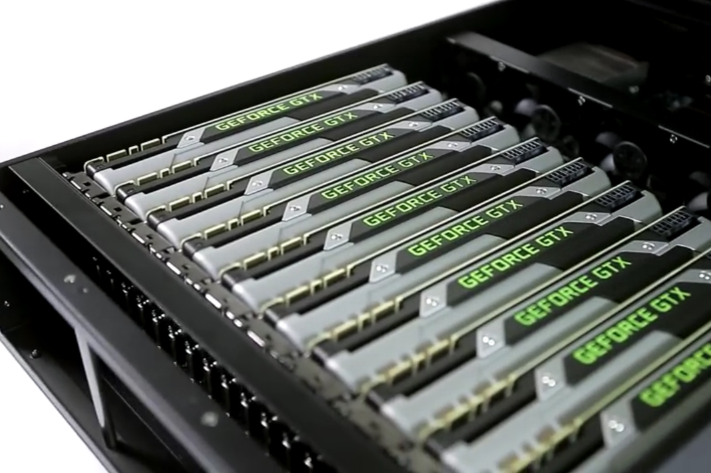
\includegraphics[width=0.8\linewidth]{2_4.png}
          \caption{GPU服务器}
    \end{figure}
\end{frame}

\begin{frame}[standout]
    Questions
\end{frame}

\end{document}

